%%% Local Variables:
%%% mode: latex
%%% TeX-master: t
%%% End:

% TODO: Poner todos los tests y problemas durante el proyecto

\documentclass{article}

\usepackage[utf8]{inputenc}
\usepackage{tikz}
\usepackage{xcolor}
\usepackage{fancyhdr}
\usepackage{fancyvrb}

\usepackage{tocloft}
\renewcommand{\cftdot}{}

\usepackage{etoolbox}
\makeatletter
\pretocmd{\section}{\addtocontents{toc}{\protect\addvspace{20\p@}}}{}{}
\pretocmd{\subsection}{\addtocontents{toc}{\protect\addvspace{10\p@}}}{}{}
\makeatother

\usepackage{wrapfig}
\usepackage{subcaption}
\usepackage{float}
% \renewcommand\familydefault{\sfdefault}


\pagestyle{fancy}
\fancyhf{}
\rhead{Sistemas de Percepción}
\lhead{}
\fancyfoot[LE,RO]{Página  \thepage}

\renewcommand{\contentsname}{Índice}

\setcounter{secnumdepth}{0}

\begin{document}

\begin{titlepage}

  \tikz[remember picture, overlay] \node[opacity=0.3,inner sep=0pt] at (current page.center){
\includegraphics[width=\paperwidth,height=\paperheight]{background8}};

  \vspace*{2cm}
  \noindent{\fontsize{32}{20}\selectfont Detección de marcadores AruCo}\\

  \vspace*{1cm}
    
  \noindent {\fontsize{18}{10}\selectfont Sistemas de Percepción}\\
  \noindent {\fontsize{16}{10}\selectfont Grupo 21}\\

  \vspace*{1cm}
  \noindent {\fontsize{14}{10}\selectfont 100363683 David Ruiz Barajas}\\
  \noindent {\fontsize{14}{10}\selectfont 100363693 Sergio Vinagrero Gutiérrez}\\

  \vspace*{2cm}
  \noindent\includegraphics[width=.5\textwidth]{/home/vinagrero/Templates/UC3M/template/logo_completo_horizontal.png}

\thispagestyle{empty}
\end{titlepage}

\tableofcontents
\newpage

\section{Introducción}
\label{introduction}

En esta memoria se detalla el proceso seguido para realizar el proyecto de detección de marcadores Aruco. Se comenzará detallando el proceso de desarrollo del algoritmo, seguido de su implementación en el código. Para finalizar, se mostrarán los problemas que han aparecido durante el proceso.\\

% Descripcion de un aruco
\begin{wrapfigure}{r}{0.3\textwidth}
  \vspace*{-1em}
  \begin{center}
    
\includegraphics[width=0.25\textwidth]{../util/aruco_images/4x4_1000-0.png}
  \end{center}
  \vspace*{-1em}  
  \caption{Marcador}
  \label{fig:marker}
\end{wrapfigure}

Los marcadores AruCo son pequeños marcadores utilizados en algoritmos de estimación de la posición. Cada marcador pose suficiente información para estos proyectos, ya que poseen 4 esquinas, suficientes para la estimación de la posición y datos codificados de manera binario.\\
Estos datos los hacen marcadores muy robustos y dan la posibilidad de aplicar algoritmos que detección y correción de errores. Estos marcadores puden ser de tamaño arbitrario, pero los utilizados en este proyecto son de 10$\times$10 cm y tienen una matriz de 6$\times$6 datos.\\
Como se puede ver en la imagen \ref{fig:marker}, los marcadores utilizados solo tienen datos en la matriz interna de 4$\times$4. Esto será de gran utilidad más adelante cuando se muestre como se guardan los datos para ser utilizados por el programa.\\

% Objetivo del proyecto
El objetivo de este proyecto es detectar dichos marcadores en cualquier posición en el espacio. Se deben detectar correctamente las 4 esquinas y la esquina principal, independientemente de la rotación del marcador. Seguidamente, se identificarán los marcadores y se dibujara una figura en 3D proyectado en el AruCo, dependiendo del identificador del marcador.

\newpage
\section{Algoritmo}

El primer paso en cualquier proceso de visión artificial es el preprocesamiento de la imagen obtenida mediante la cámara. Tras obtener una imagen de la camara, es necesario convertirla a escala de grises.


Por lo tanto, el algoritmo quedaria resumido de la siguiente manera:

\begin{enumerate}
\item Aplicación de threshold a la imagen obtenida.

\item Busqueda de contornos. Se han encontrado mas contornos de los necesarios, por lo que hay que eliminarlos.
  \begin{enumerate}
  \item Eliminación cualquier contorno que no sea rectangular.
  \item Eliminamos los contornos que no cumplan con las especificaciones de tamaño.
  \item Eliminamos contornos que no tienen un contorno dentro de ellos.
  \end{enumerate}

\item Identificación del marcador.
  \begin{enumerate}
  \item Obtención de la imagen frontal del marcador mediante homografía.
  \item Aplicación de threshold utilizando Otsu a la imagen frontal.
  \item Lectura de los 16 bits internos del marcador.
    \item Comparación del diccionario leido con la lista predefinida. Si no hay ninguna correspondencia el marcador es eliminado.
    \end{enumerate}

  \item Proyección de los puntos 3D en la imagen obtenida inicialmente.
  \item Dibujo del contorno, primer vértice figura correspondiente de cada marcador en la imagen.
\end{enumerate}


% Justificacion del algoritmo. Por que lo hace de esa manera.
\section{Implementación}

\subsection{Segmentación de la imagen}
Hay varias maneras de aplicar el threshold a la imagen de la cámara. Como los marcadores son blancos y negros, la mejor opción será aplicar un threshold binario. No obstante, este proceso no es perfecto, ya que para cada frame, debemos calcular el valor para segmentar la imagen para poder distinguir correctamente las partes blanca y negra del marcador.\\
Este proceso es costoso computacionalmente dado que hay que calcular el valor de segmentacion para cada frame y en el caso de que haya varios marcadores en la imagen, y esten a distintos niveles de iluminación, este proceso no buscara el valor ideal, por lo que es necesario utilizar otro método.\\

Se ha dedicido aplicar un thresold local, conocido en opencv como \textit{adaptiveThreshold}. De esta manera, el valor de segmentación es calculado para regiones más pequeñas, evitando el problema de encontrar el valor ideal al haber multiples marcadores. Además, conseguimos hacer que el sistema sea invariante ante cambios de iluminación.\\

% Dos imagenes: Una de threshold y otra de adaptiveThreshold
Se puede observar la diferencia entre ambas funciones en las dos imágenes.
\begin{figure}[H]
  \centering
  \begin{subfigure}[c]{0.45\textwidth}
    \centering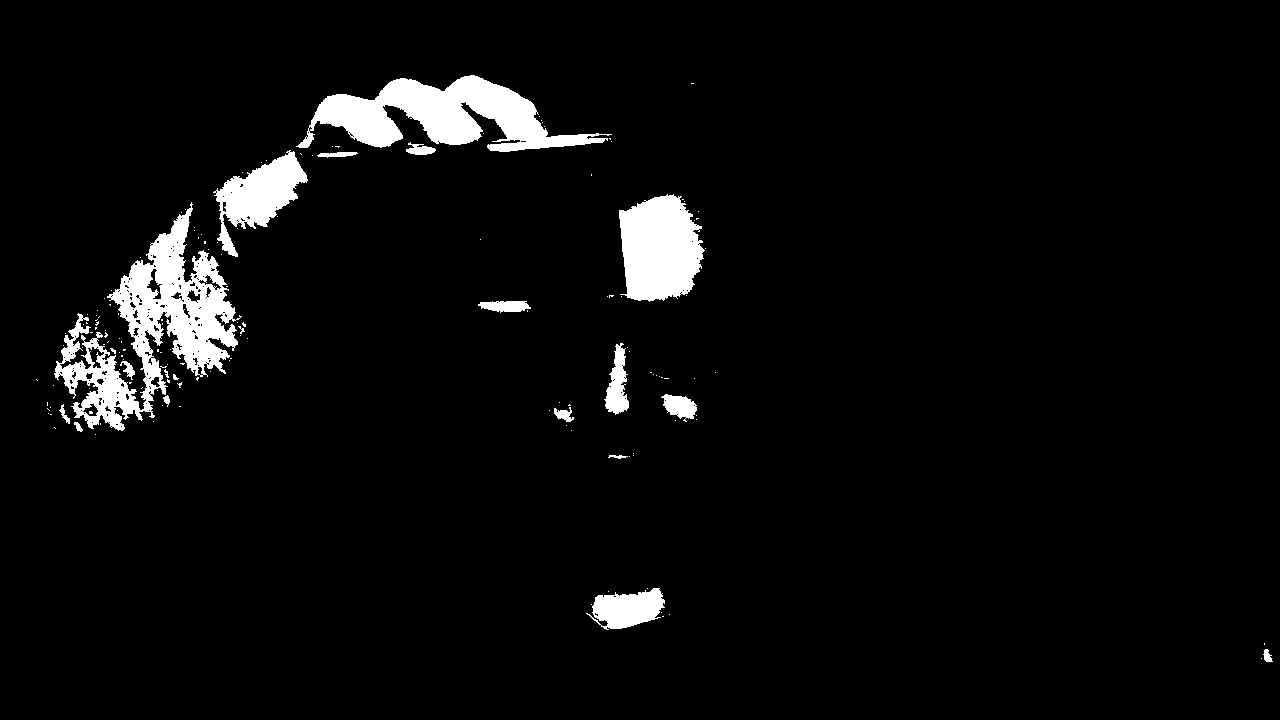
\includegraphics[width=\textwidth]{threshold.png}
    \caption{Threshold}
    \label{fig:normalthresh}
  \end{subfigure}
  \hfill
  \begin{subfigure}[c]{0.45\textwidth}
    \centering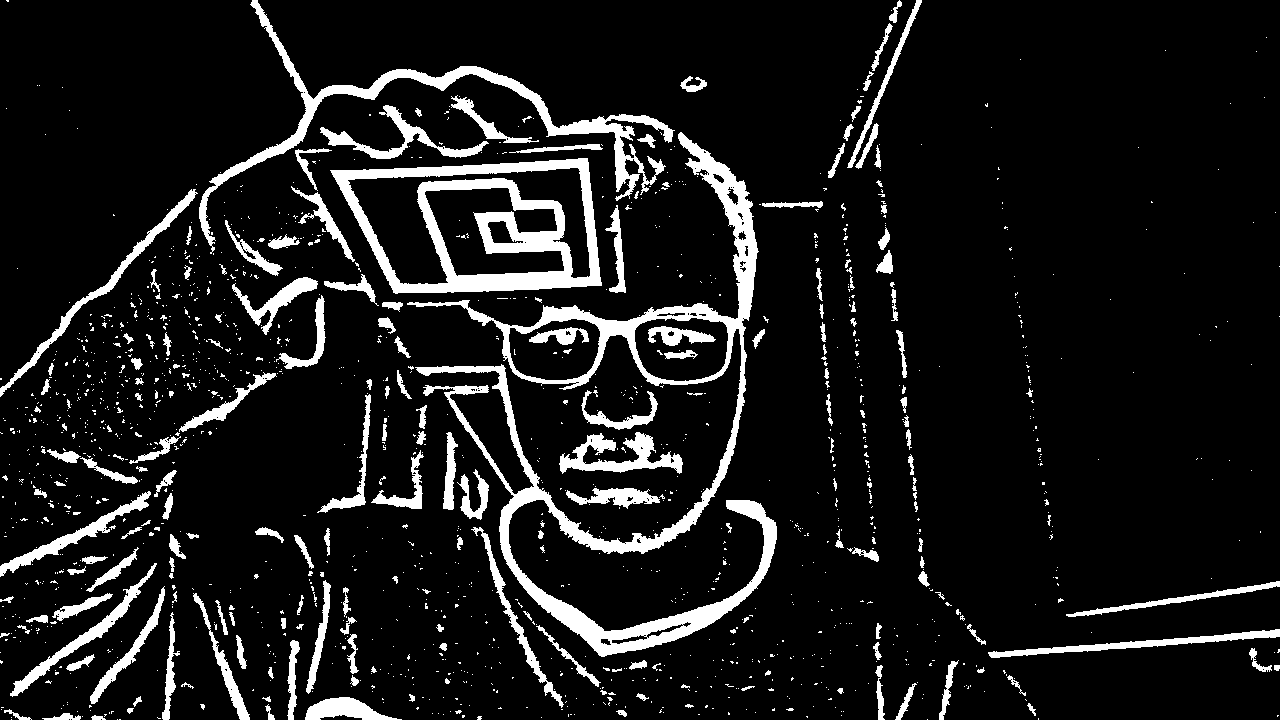
\includegraphics[width=\textwidth]{adaptive_threshold.png}
    \caption{adaptiveThreshold}
    \label{fig:adaptivethresh}
  \end{subfigure}
  \caption{Diferencia entre los dos tipos de threshold}
  \label{fig:diffthresh}
\end{figure}

% Deteccion de contornos
\subsection{Detección de contornos}
Se realizará ahora una búsqueda de todos los contornos en la imagen binarizada. Uno de los problemas de utilizar threshold local, es el ruido que este genera. Se puede ver en la imagen~\ref{fig:adaptivethresh} como obtenemos ruido impulsional en la imagen de salida. Este generará muchos contornos cuando se busquen marcadores, por lo que es recomendable eliminarlo. Para eliminarlo se pueden aplicar dos procesos:

\begin{itemize}
\item Aplicación de filtro de la mediana.
\item Una vez calculados los contornos, ignorar aquellos cuya area no supere un umbral.
\end{itemize}

Al realizar las pruebas con los dos metodos, se comprobó que realizar una pasada con el filtro de la mediana realentiza el algoritmo más que si solo se ignoran ciertos contornos.\\

Se procede ahora a buscar todos los contornos en la imagen binarizada. Otro sesgo de posibles marcadores se realiza en este paso, ya que podemos aproximar el perímetro del contorno detectado a una figura cerrada y convexa. En el caso de que dicha figura resultante no tenga cuatro lados, descartamos la figura ya que no puede ser un marcador. Conseguimos asi analizar solo aquellos contornos que tengan forma rectangular o cuadrada.\\
OpenCV permite agrupar los contornos detectados en una jerarquía. De esta manera, podemos referirnos a un contorno mediante su contorno padre o su contorno hijo.
Esto es de gran utilidad, ya que como podemos ver en la imagen~\ref{fig:marker} y en la imagen~\ref{fig:adaptivethresh}, el marcador AruCo pose dos contornos: el paso de negro a blanco del marco y la información codificada en el propio marcador. Gracias a esto, se descartan todos aquellas figuras rectangulares que no posean dentro otro contorno.\\
Es necesario tener en cuenta que incluso con las condiciones establecidas hasta ahora, se han podido detectar figurar que no sean arucos, siempre y cuando sean rectangulares y posean otro contorno dentro. El último sesgo se realizará posteriormente, antes de dibujar la figura en la pantalla.\\

% Imagen plana del marcador
\subsection{Extracción del marcador}
Para facilitar la extracción de los datos del marcador, se procede ahora a obtener una imagen plana de dicho marcador. Para ello utilizaremos dos planos homograficos: el plano formado por los 4 vértices del marcador en la primera imagen obtenida por la cámara y un plano creado como si se estuviese viendo el marcador de frente.\\

Este proceso se realiza sobre la primera imagen obtenida por la cámara ya que, como se ha explicado anteriormente, la imagen binarizada contiene demasiado ruido.\\

Para cada imagen frontal del aruco, se segmenta la imagen utilizando Otsu. Como la imagen frontal del marcador se obtiene de la imagen original, hay que segmentar la imagen. Otsu nos permite encontrar el punto ideal para segmentar cada marcador, ya que como se ha indicado anteriormente, debido a cambios de iluminacion en el entorno y posiciones de los marcadores, cada aruco tendrá un punto de segmentación distinto.

% Identificación del marcador
\subsection{Identificación del marcador}
Como se ha explicado en la sección \ref{introduction}, la información util de los marcadores está codificada en una matriz 4$\times$4 en el centro del marcador.
Para extraer dicha matriz, se trabaja sobre la imagen plana que se ha obtenido anteriormente. Para facilitar la extracción de datos, se ajusta el tamaño de esta imagen a una de 6$\times$6 píxeles, donde cada pixel corresponde a un bit del marcador.\\

Una vez extraidos los 16 valores, se procede a la comparación de esta matriz con una lista de matrices predefinidas.

\noindent
\begin{minipage}{0.6\textwidth}
  Para generar estos valores automaticamente, se ha escrito un script en Python.\\ Dicho script recibe la ruta al directorio con los marcadores, y genera el output mostrado a la derecha para cada marcador encontrado.\\

  El valor 255 corresponde a un bit blanco y el 0 a uno negro. Se crean 4 matrices, una para cada angulo de rotacion del marcador y se guardan en sentido horario. Esto será muy util a la hora de dibujar el primer vértice del marcador, lo cual se detallará más adelante.\\
  Para este proyecto se han utilizado 10 marcadores aruco, por lo que la lista de diccionarios contiene 40 matrices.\\

  Se ha escogido este método de guardar la información de cada marcador dado que utiliza pocos recursos en memoría (40 matrices $\times$ 16 valores $\times$ 1 byte/número = \textbf{640 bytes}) y se evitar tener que rotar una matriz 4 veces por iteración, lo que incrementaría la complejidad del programa.
  
\end{minipage}%
\hfill
\begin{minipage}{0.35\textwidth}
\begin{center}
\begin{BVerbatim}
// Marker 1
{{0  , 0  , 0  , 0  }, 
 {255, 255, 255, 255}, 
 {255, 0  , 0  , 255}, 
 {255, 0  , 255, 0  }},
                       
{{0  , 255, 255, 0  }, 
 {0  , 255, 0  , 255}, 
 {0  , 255, 0  , 0  }, 
 {0  , 255, 255, 255}},

{{0  , 255, 0  , 255},
 {255, 0  , 0  , 255},
 {255, 255, 255, 255},
 {0  , 0  , 0  , 0  }},

{{255, 255, 255, 0  },
 {0  , 0  , 255, 0  },
 {255, 0  , 255, 0  },
 {0  , 255, 255, 0  }},
\end{BVerbatim}
\end{center}
\end{minipage}

\vspace*{1em}

Cuando la matriz calcula previamente coindice con una de la lista generada, el marcador se identifica con el íncide de la matriz en la lista de diccionarios. En el caso de que el marcador detectado no coincida con ningún diccionario de la lista se le asigna el id -1. Este es el ultimo de los sesgos realizados a la imagen para que finalmente solo se consiga dibujar los marcadores.\\

No obstante, este método requiere conecimiento a priori de los marcadores a detectar, por lo que no se pueden añadir marcadores nuevos durante la ejecucion del programa.

% Calculo de puntos 3D
\subsection{Cálculo de puntos 3D}
Esta es la última etapa del proceso. Aquí dibujaremos todos aquellos marcadores cuyo id sea distinto de -1. De esta manera solo dibujaremos en la pantalla arucos reales.\\

Junto a la lista de diccionarios predefinidos, se ha creado un mapa de valores que relaciona el id del marcador con una figura en 3D para dibujar. Actualmente, el código permite el dibujo de un cubo, una pirámide, una pirámide invertida y una pirámide apoyada en un lado. Añadir figuras nuevas al sistema seria tan facil como asignarles un aruco, buscar los puntos 3D de dicha figura y poner el código para conectar los vértices de dicha figura.\\

Para este paso necesitaremos lo siguiente:
\begin{itemize}
\item Matriz de la cámara y de los coeficientes de distorsión.
\item Puntos 2D del marcador en la imagen.
\item Puntos 3D de la cara inferior del marcador.
\item Puntos 3D del objeto a proyectar en la imagen.
  \end{itemize}

  Con estos datos, OpenCV encuentra la matriz de rotación y de traslación para proyectar los puntos 3D de la cara inferior del marcador en 2D en la imagen de la cámara. De esta manera, tenemos una manera de trasladar, o proyectar, puntos en 3D en la imagen de la cámara.

  \subsection{Obtención de fps}

  Una vez el programa funciona correctamente, es necesario comprobar la velocidad a la que funciona, dado que existe el requerimiento de ejecución en tiempo real.\\

Si leemos las imagenes de un video, podemos acceder a los metadatos de este y ver los frames a los que se reproduce dicho video. Los metadatos de los fps se acceden mediante el atributo \textit{CV\_CAP\_PROP\_FPS}. Sin embargo, esto solo nos permite conocer la velocidad a la que reproduce el video, pero no la velocidad a la que se procesa.\\
  
Para solventar este problema se ha creado un contador básico mediante el uso de dos variables. Se calcula el tiempo que hay de diferencia entre ambas una vez se hayan analizado un numero determinado de frames. Se ha escogido 30 frames como éste número, ya que la mayoría de las webcams no graban a más de 30 fps.
  
 % TODO: Añadir imagenes de las figuras dibujadas
\section{Resumen}

Como se puede ver, a lo largo de este proyecto se han utilizado la mayoría de técnicas de procesamiento de imágenes vistas en clase.
También se ha podido ver de primera mano la importancia de un buen preprocesamiento de la imagen, ya que son los cimientos sobre los que se realizarán las siguientes etapas.

\end{document}
